%
% jikken.cls を使った LaTeX 報告書のひな型ファイル
%
% 表紙だけを作るのにも報告書全体を作るのにも使える
%

\documentclass[indiv]{jikken}   % 実験報告用クラスファイル (jikken.cls) が必要
\usepackage[dvipdfmx]{graphicx}  %pngファイルを貼り付けるのに必要
\usepackage[dvipdfmx]{color}
\usepackage{listings, jlisting}
\usepackage{color}
\usepackage{float}
\usepackage{ascmac}
\usepackage{amsmath}

\lstset{
	%プログラム言語(複数の言語に対応,C,C++も可)
 	language = R,
 	%背景色と透過度
 	backgroundcolor={\color[gray]{.90}},
 	%枠外に行った時の自動改行
 	breaklines = true,
 	%自動改行後のインデント量(デフォルトでは20[pt])	
 	breakindent = 10pt,
 	%標準の書体
 	basicstyle = \ttfamily\scriptsize,
 	%コメントの書体
 	commentstyle = {\itshape \color[cmyk]{1,0.4,1,0}},
 	%関数名等の色の設定
 	classoffset = 0,
 	%キーワード(int, ifなど)の書体
 	keywordstyle = {\bfseries \color[cmyk]{0,1,0,0}},
 	%表示する文字の書体
 	stringstyle = {\ttfamily \color[rgb]{0,0,1}},
 	%枠 "t"は上に線を記載, "T"は上に二重線を記載
	%他オプション:leftline,topline,bottomline,lines,single,shadowbox
 	frame = TBrl,
 	%frameまでの間隔(行番号とプログラムの間)
 	framesep = 5pt,
 	%行番号の位置
 	numbers = left,
	%行番号の間隔
 	stepnumber = 1,
	%行番号の書体
 	numberstyle = \tiny,
	%タブの大きさ
 	tabsize = 4,
 	%キャプションの場所("tb"ならば上下両方に記載)
 	captionpos = t,
    %空白を表示するかどうか
    showstringspaces = false,
}

\setcounter{secnumdepth}{3}  %目次のために必要

%%% 通常は書き換え不要
%\renewcommand{\科目名}{情 報 工 学 実 験~~I・II}
\renewcommand{\作成日}{\today}
\renewcommand{\学年}{3}

\newcommand{\本年}{令和2年}
\newcommand{\次年}{令和3年}

%%% 必要に応じて書き換える
\renewcommand{\実験名}{アナログ/ディジタルフィルタによる信号処理}

%%% {平成 \num 年 \num 月 \num 日} を実施日に書き換える(不要なら {} にする)
%%% \num 月 \num 日 を実施日に書き換える
\newcommand{\実施日1}{\本年 4 月 11 日}
\newcommand{\実施日2}{\本年 4 月 18 日}
\newcommand{\実施日3}{\本年 4 月 25 日}
\newcommand{\実施日4}{\本年 5 月 9 日}
\newcommand{\実施日5}{\次年 5 月 16 日}
\newcommand{\実施日6}{\次年 5 月 23 日}
\newcommand{\実施日7}{\次年 5 月 30 日}

%%% \groupnum を報告者の班番号に書き換える
\newcommand{\班番号}{\groupnum}

%%% {\samplenum}{\samplename} を番号と氏名に書き換える(不要なら {}{} にする)
\newcommand{\報告者}{\番号と氏名{421858}{若山陽向}}
\newcommand{\実験者1}{\番号と氏名{\samplenum}{\samplename}}
\newcommand{\実験者2}{\番号と氏名{\samplenum}{\samplename}}
\newcommand{\実験者3}{\番号と氏名{\samplenum}{\samplename}}
\newcommand{\実験者4}{\番号と氏名{\samplenum}{\samplename}}
\newcommand{\実験者5}{\番号と氏名{\samplenum}{\samplename}}
\newcommand{\実験者6}{\番号と氏名{\samplenum}{\samplename}}
\newcommand{\実験者7}{\番号と氏名{\samplenum}{\samplename}}

%%%%%%%%%%%%%%%%%%%%%%%%%%%%%%%%%%%%%%%%%%%%%%%%%%%%%%%%%%%%%%%%%%%%%%%%%%%%%%

\begin{document}

\表紙  % 報告書の表紙を作る

%%% 報告書全体を作るなら以下を書き換える

\section{目的}     
実験に必要な環境整備としてOctaveとRのインストール状況を確認し、それぞれのソフトの基本的な操作法をマスターする。

\section{解説}
Octaveについてはディジタル信号処理の授業の1回目(2020/10/6)で解説済みのため、Rの基本操作について解説する。
OctaveやRを使用して、与えられたデータ(xlsxまたはcsv形式)を処理し、指定された形式のグラフを作成し、レポートにまとめる。

\section{実験方法}
気象庁のホームページから日本の平均気温の変化に関するデータをcsv形式でダウンロードし、プロットされた図をレポートに埋め込む。

\section{実験結果}

\subsection{実験課題1}

与えられた課題に対してRで実行できる以下のようなスクリプトを作成した

\begin{lstlisting}[basicstyle=\ttfamily\footnotesize, caption=Rのスクリプト]
pdf("3年前期AD信号処理1(R).pdf")
data = read.csv("mon_jpn.csv")
data_jan = subset(data, , c(YEAR, JAN))
plot(data_jan, type="b", xlab = "Year", ylab="Difference from the average temperature(1981-2010)[degree]")
lm_jan = lm(JAN~YEAR, data = data_jan)
abline(lm_jan)

#トレンド(100年あたりの変化量)について
#まず、lm_janの傾きは、lm_janを入力した時の返り値

#> lm_jan

#Call:
#lm(formula = SEP ~ YEAR, data = data_jan)

#Coefficients:
#(Intercept)         YEAR  
#  -23.60301      0.01185  

#より、CoefficientsのYEARの方に注目して0.001185だと分かります。
#これは1年分の変化量に相当するので、トレンド(100年あたりの変化量)はこれを100倍して
#1.185だと分かります。
dev.off()
\end{lstlisting}

プロットされたグラフを図\ref{plot1}に示す。
\begin{figure}[H]
    \begin{center}
     \resizebox{12cm}{!}{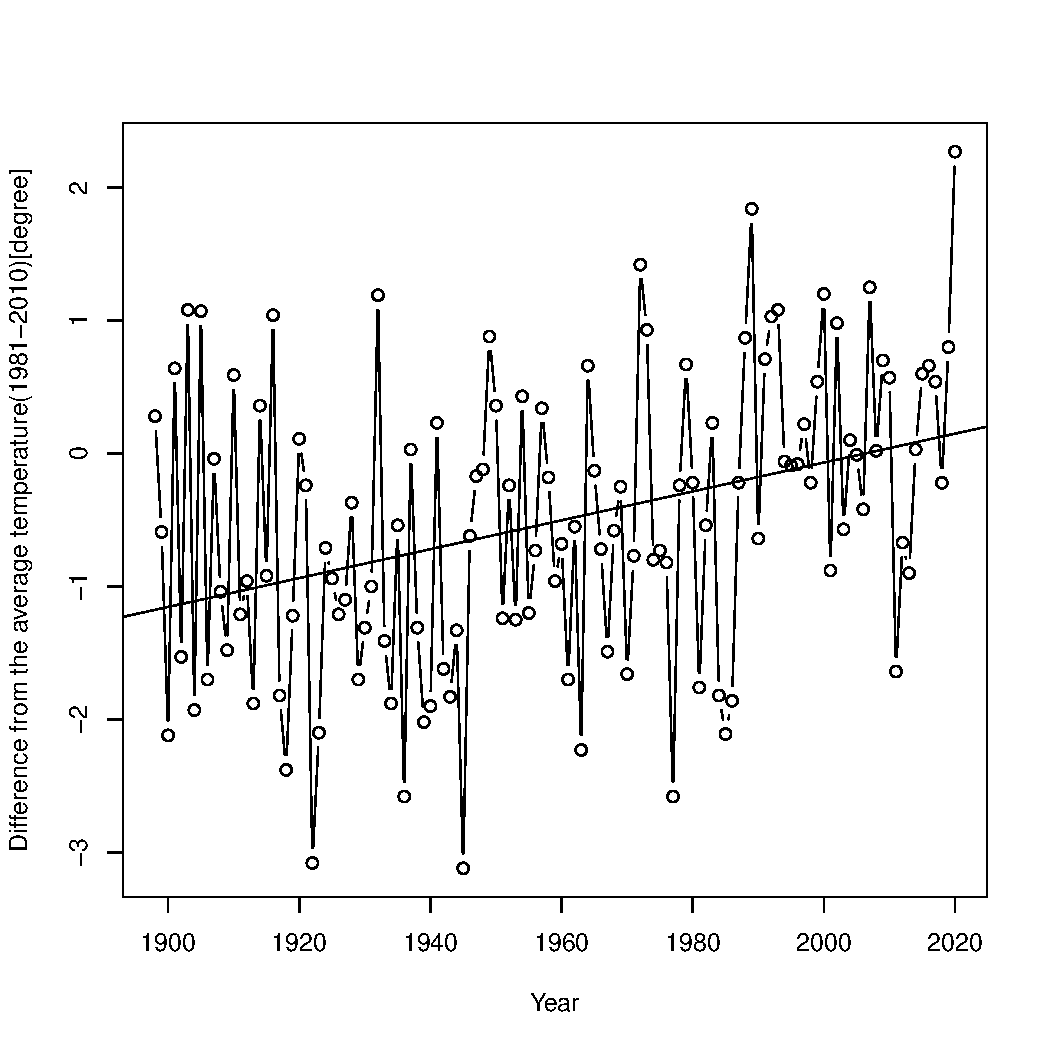
\includegraphics{ADtrans1_R.pdf}}
     \caption{Rによる作図結果}\label{plot1}
    \end{center}
\end{figure}

\subsection{実験課題2}

与えられた課題に対してOctaveで実行できる以下のようなスクリプトを作成した。

\begin{lstlisting}[basicstyle=\ttfamily\footnotesize, caption=Octaveのスクリプト]
#csvファイルを読み取る
data = csvread("mon_jpn.csv");

#YEARに2行1列目~124行1列目(つまり1898年~2020年)を代入
YEAR = data(2:124,1);

#JANに2行2列目~124行2列目(つまり1月の平均気温偏差)を代入
JAN = data(2:124,2);

hold on;
#プロットする
plot(YEAR, JAN, 'b-o');
xlabel("Year");
ylabel("Difference from the average temperature(1981-2010)[degree]");
set(gca,'fontsize',5)
grid;

%{
ここで、Rにおける結果
#> lm_jan

#Call:
#lm(formula = SEP ~ YEAR, data = data_jan)

#Coefficients:
#(Intercept) YEAR
# -23.60301 0.01185
を用いて、近似線の傾きと切片が分かったので、これもプロットする。
%}
y = 0.01185 * YEAR -23.60301;
plot(YEAR, y);
hold off;

print('ADtrans1_Octave.pdf', '-dpdf');
\end{lstlisting}

プロットされたグラフを図\ref{plot2}に示す。

\begin{figure}[H]
    \begin{center}
     \resizebox{12cm}{!}{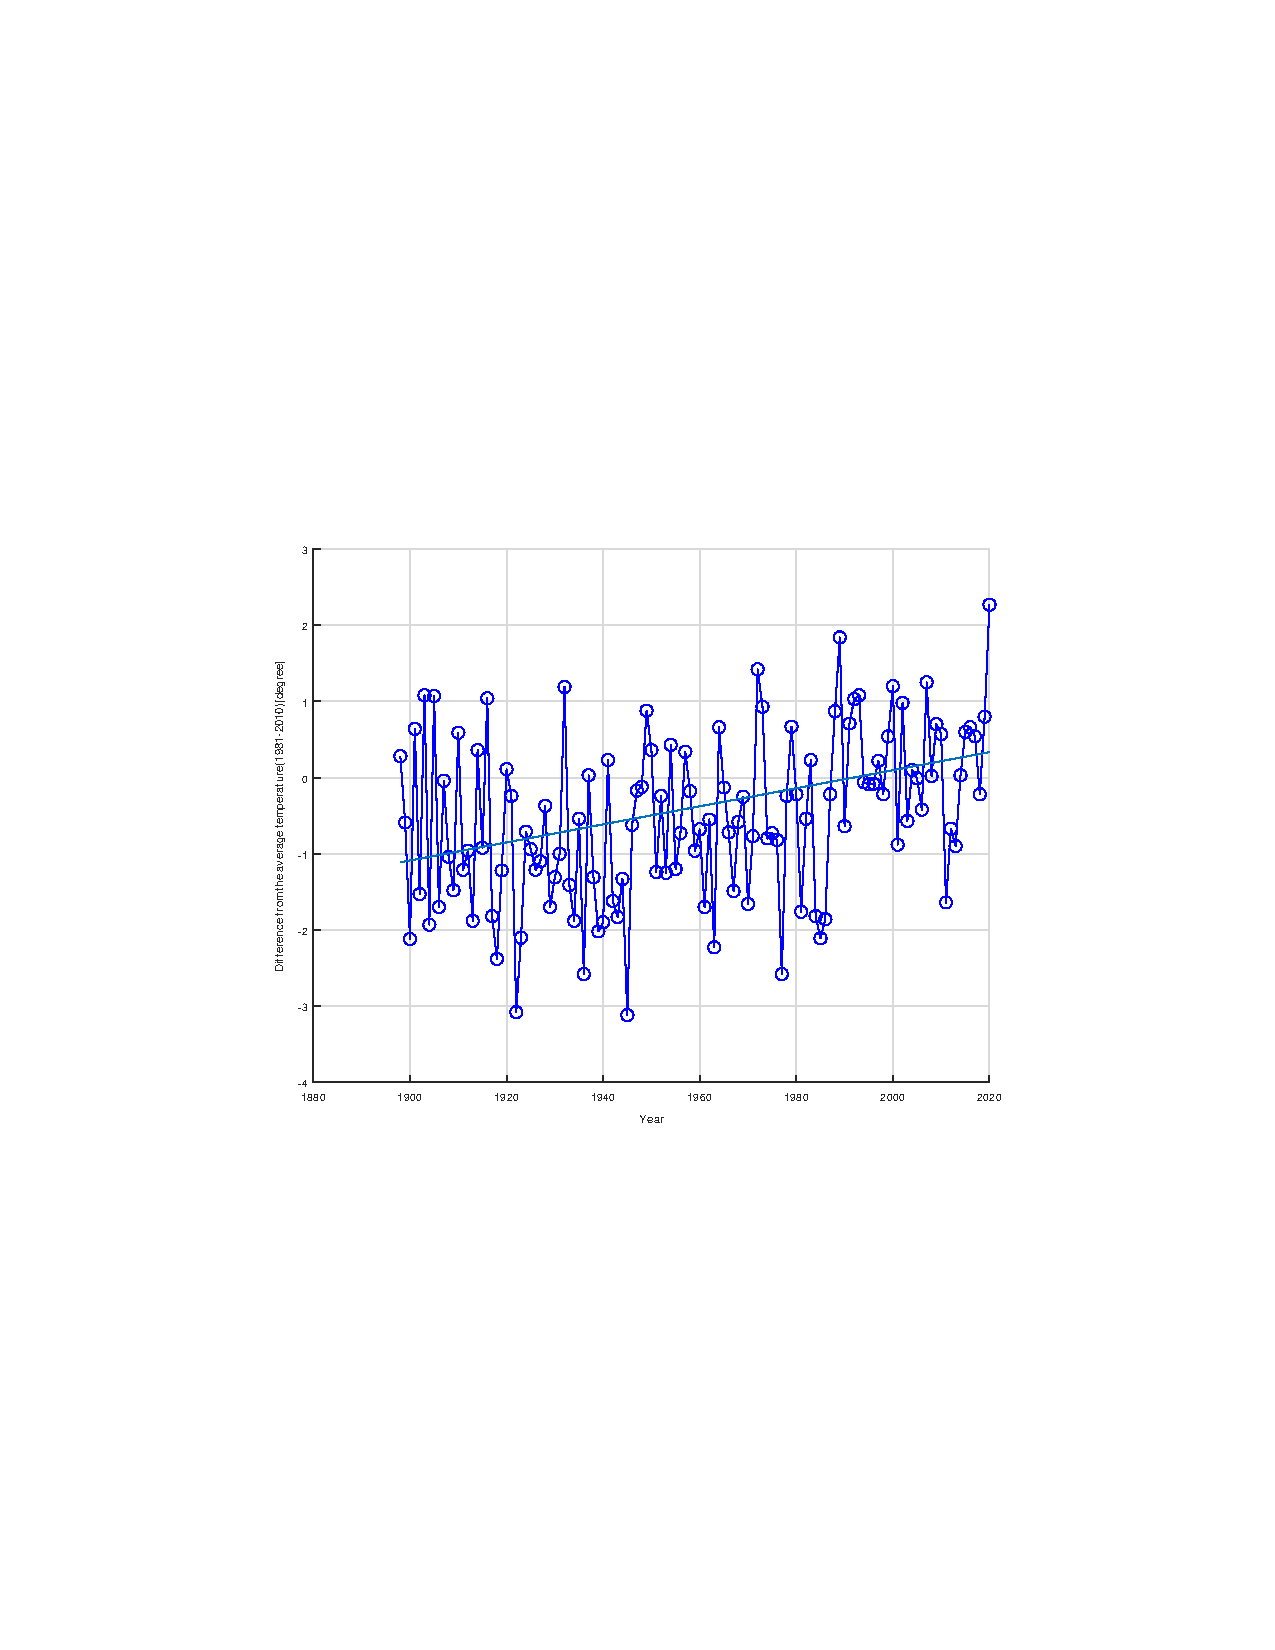
\includegraphics{ADtrans1_Octave.pdf}}
     \caption{Octaveによる作図結果}\label{plot2}
    \end{center}
\end{figure}

\section{感想}
慣れていないからかも知れないが、\verb|R|より\verb|Octave|の方が使いやすいと感じた。


\begin{thebibliography}{9} % 参考文献
\bibitem{Yamada2020}
気象庁HP, 『日本の月平均気温偏差』, \\\verb| http://www.data.jma.go.jp/cpdinfo/temp/list/mon_jpn.html | (2020/10/7 アクセス).
\end{thebibliography}

\end{document}